
%%------------------------
%% Oct 9, 2021
%% Y. Lee
%% (D) Interactive Geometry
%% 1. Geometric constructions
%% Source of this Activity: Exploring Conic Sections with The Geometer’s SketchPad © 2002 Key Curriculum Press
%%------------------------

\documentclass[11pt]{article}
\usepackage{latexsym,amssymb}%,times,mathptm}
\usepackage{amsmath}
\usepackage{amscd}
\usepackage{makeidx}
\usepackage{enumerate}
\usepackage{graphicx}

\input xypic
\baselineskip=55pt


\textwidth=6.5in
\hoffset=-0.8 in
\voffset=-0.5 in
\textheight=8.3 in


\newcommand{\mi}[1]{#1\index{#1}}
\newcommand{\llar}{-\kern-5pt-\kern-5pt\longrightarrow}



\def\ann{\mbox{\rm ann}}
\def\Ass{\mbox{\rm Ass}}


\begin{document}

\begin{center}
{\bf MAT 140 \quad Computational Tools for Mathematics and the Sciences}

\end{center}

\medskip
\noindent {Chapter:  \quad Geometry}

\smallskip

\noindent {Technology: GeoGebra}

\smallskip

\noindent {Section:  \quad \quad Construction of Parabola }

\smallskip

\noindent {Activity time: 50 minutes}


\vspace{0.2 in}


\noindent {\bf I. Preamble}

\smallskip

\noindent In this lab, you will learn how to use GeoGebra to construct a geometric object and how to apply the distance definition of parabola to analyze your construction. Remember, \textbf{a parabola} is the set of points equidistant from a fixed point (the focus) and a fixed line (the directrix). 
\vspace{0.2 in}

In fact, you can create a parabola with nothing more than a sheet of wax (or plain) paper and a single point on the page! This video in the link will show you how one can fold a paper to create a parabola (https://www.youtube.com/watch?v=GdJlbNweSVY). %%This video may not be the best one out there. 
\vspace{0.2 in}

But, creasing your paper takes some work. Folding one or two sheets is fun, but what would happen if you wanted to continue testing many different locations for point A? You’d need to keep starting over with fresh paper, folding new sets of creases. Technology can streamline your work. With just one set of creases, you can drag the Focus point to new locations and watch the crease lines adjust themselves instantaneously.


\vspace{0.2 in}

\noindent {\bf II. Constructing a GeoGebra model}




\begin{center}
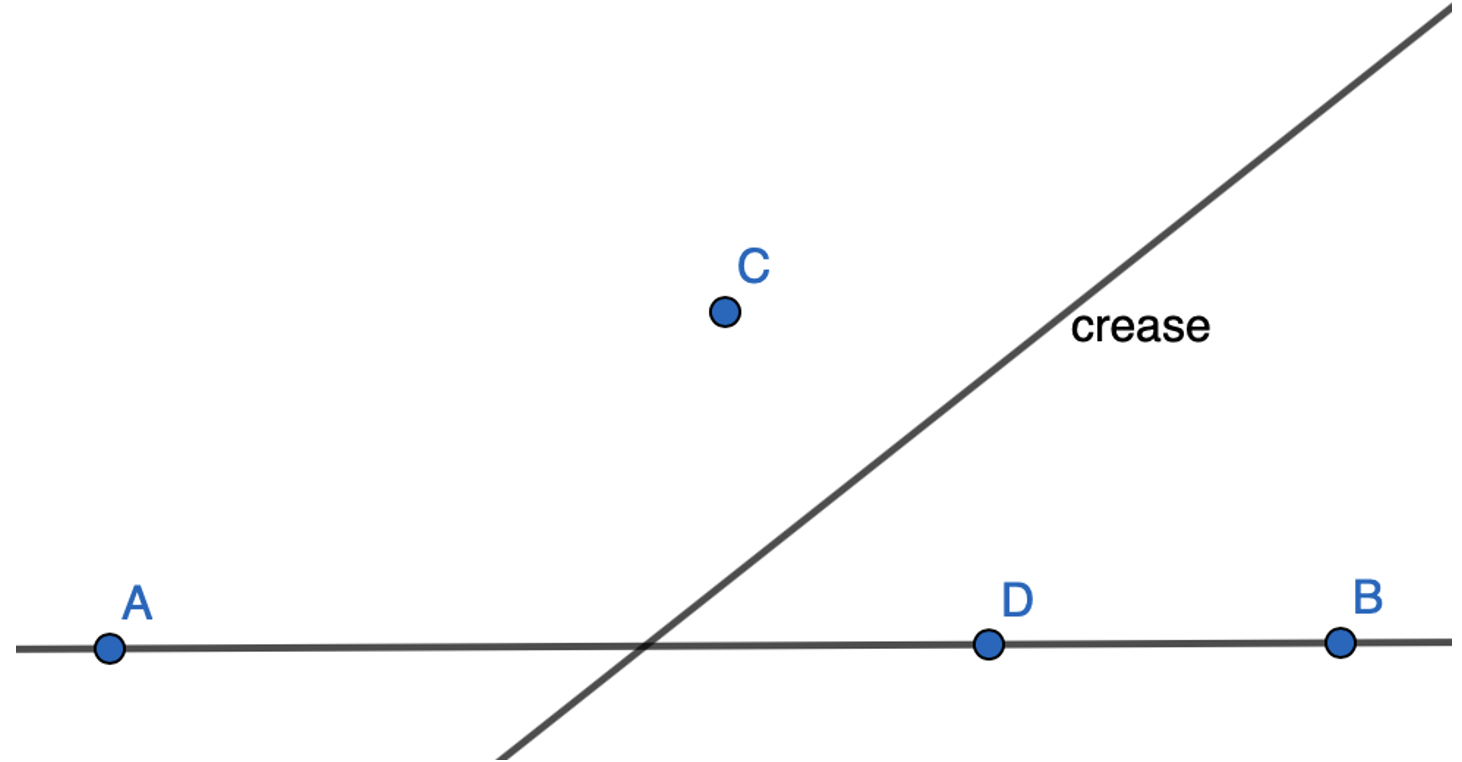
\includegraphics[width=0.5\textwidth]{figure1.png}
\end{center}

\begin{enumerate}[(1)]
\item In GeoGebra, use the Line tool to draw a horizontal line near the bottom of the screen. This line AB represents the bottom edge of the paper.
\item Draw a point C above the line, roughly centered between the left and right edges of the screen.	 	
\item Construct a point D on the horizontal line.
\item Construct the “crease” formed when point D is folded onto point C.
\item Drag point D along its line. If you constructed your crease line correctly, it should adjust to the new locations of point D.
\item Select the crease line and choose "Show trace" from the right-click menu.
\item Drag point D along the horizontal line to create a collection of crease lines.
\item To see other cases, clear all traces and drag point C to a different location.
\item Drag point D to create another collection of crease lines.
\end{enumerate}

\smallskip

\noindent Retracing creases for each location of point C is certainly faster than folding a paper. GeoGebra’s powerful "Show trace" feature and dragging capability make it possible to observe various cases of folding a paper efficiently and explore the properties of geometric objects you are observing.




\vspace{0.2 in}

\noindent {\bf III. Questions}

\begin{enumerate}[(A)]
\item How does the appearance of the curve change as you move point C closer to the horizontal line?

\item How does the appearance of the curve change as you move point C away from the horizontal line?


\end{enumerate}

\vspace{0.2 in}

\noindent {\bf IV. Playing detective}

\smallskip

\noindent Each crease line on your paper touches the parabola at exactly one point. Another way of saying this is that each crease is tangent to the parabola. By engaging in some detective work, you can locate these tangency points and use them to construct just the parabola without its creases.




\begin{center}
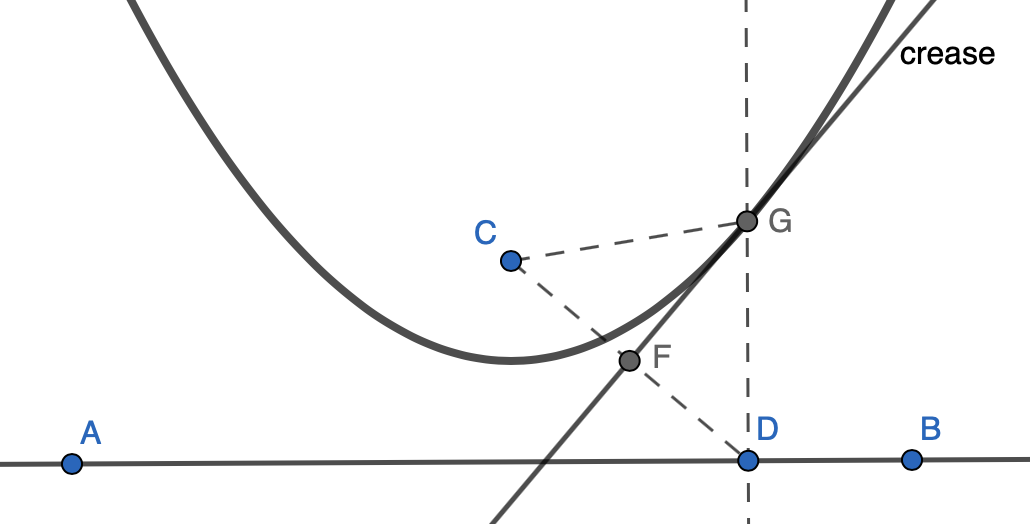
\includegraphics[width=0.5\textwidth]{figure2.png}
\end{center}

\begin{enumerate}[(1)]

\item The exact point of tangency lies at the intersection of two lines—the crease line and another line not shown here. Construct this line in your sketch as well as the point of tangency, point G.

\item The construction above seems to generate a parabola. Can you convince others that it does? Try developing argument on your own or work through the following steps and questions. The picture above should resemble your GeoGebra construction. Line FG (the perpendicular bisector of segment CD) represents the crease line formed when point D is folded onto point C. Point G sits on the curve itself.
	
\end{enumerate}

\vspace{0.2 in}

\noindent {\bf V. Questions}

\begin{enumerate}[(A)]
\item Assuming point G traces a parabola and using the distance definition of parabola, which two segments must you show equal in length?

\item Use a triangle congruence theorem to show that $$\triangle {CFG} \cong \triangle {DFG}.$$

\item Use the distance definition of a parabola and the result from the question above to show that point G traces a parabola. (Remember, a parabola is the set of points equidistant from a fixed point (the focus) and a fixed line (the directrix).)

\end{enumerate}

\end{document}

\noindent Approved by the MDCC, .

\noindent Approved by the department of mathematics, .


